\documentclass[14pt, hyperref = {colorlinks}]{beamer}
\usepackage[T2A]{fontenc}
\usepackage[utf8]{inputenc}
\usepackage[english,russian]{babel}
\usepackage[colorlinks]{hyperref}
\usepackage{amssymb,amsfonts,amsmath,mathtext}
\usepackage{cite,enumerate,float,indentfirst}

\usepackage{xmpmulti}
%\usefonttheme{structurebold}     % Font theme: serif
%\usepackage{ccfonts}     % Font family: Concrete Math
%\usepackage[T1]{fontenc} % Font encoding: T1

\usetheme{Boadilla}

\hypersetup{
	colorlinks=true,
	linkcolor=blue,
	filecolor=magenta,      
	urlcolor=cyan,
}
\usecolortheme{seahorse}

\setbeamercolor{footline}{fg=blue}
\setbeamertemplate{footline}{
	\leavevmode%
	\hbox{%
		\begin{beamercolorbox}[wd=.333333\paperwidth,ht=2.25ex,dp=1ex,center]{}%
			А.Е. Требушинин
		\end{beamercolorbox}%
		\begin{beamercolorbox}[wd=.333333\paperwidth,ht=2.25ex,dp=1ex,center]{}%
			Новосибирск, 2019
		\end{beamercolorbox}%
		\begin{beamercolorbox}[wd=.333333\paperwidth,ht=2.25ex,dp=1ex,right]{}%
			Стр. \insertframenumber{} из \inserttotalframenumber \hspace*{2ex}
	\end{beamercolorbox}}%
	\vskip0pt%
}

\newcommand{\itemi}{\item[\checkmark]}

\title{\small{Разработка рентгенооптических трактов экспериментальных станций первой очереди проекта ЦКП «СКИФ»}}

\author{\small{%
		\emph{Докладчик:}~Требушинин Андрей\\%
		\emph{Руководитель:}~к.ф.-м.н.~Я. В. Ракшун}\\%
	\vspace{30pt}%
	Институт Ядерной Физики
	\vspace{-15pt}%
}

\date{
\includegraphics[width=0.1\linewidth]{pic/logo.jpg} \hspace{20pt}
	
\includegraphics[width=0.2\linewidth]{pic/SKIFlogo.png}\\
	
	\vspace{5pt}% 
	\small{Новосибирск, 2019}}

\begin{document}

\maketitle


\small
\begin{frame}
\frametitle{Цель работы}\label{t1}
\begin{center}
	Создание проекта экспериментальных стаций первой очереди проекта <<СКИФ>>
\begin{itemize}
	\item Моделирование \textbf{вставных устройств} \\(ондуляторы, вигглеры)
  	\item Моделирование \textbf{оптических элементов} \\(апертуры, монохроматоры, фокусирующие зеркала)
  	\item Создание \textbf{среды для обмена информаций} по проектированию
	\item Координация работы между исследовательскими группами разных институтов (ИЯФ, Институт катализа и д.р.)
\end{itemize}
\end{center}
\end{frame}

\small
\begin{frame}
\frametitle{План презентации}\label{t1}
\begin{center}
		\begin{itemize}
		\item Необходимость источников СИ в России
		\item Структура проектного офиса ЦКП <<СКИФ>>
		\item Обзор источников излучения для станций
		\item Оптические схемы станций
		\item Обсуждение результатов	
		\item Благодарности 
	\end{itemize}
\end{center}
\end{frame}

\iffalse
\small
\begin{frame}
\frametitle{Окружности и прямые}\label{t1}
\begin{figure}[h]
	\center{Синхротронный источник}
	\begin{minipage}[h]{0.50\linewidth}
		\center{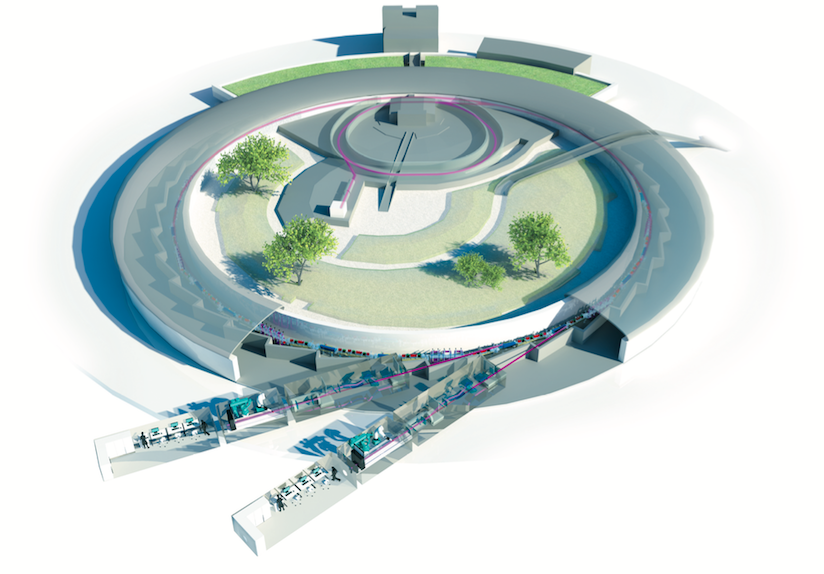
\includegraphics[width=0.99\linewidth]{pic/synchrotron.png}}
		%http://www.irtnanoelec.fr
	\end{minipage}

	\hfill
	\center{Лазер на свободный электронах}
	\begin{minipage}[h]{0.50\linewidth}
		\center{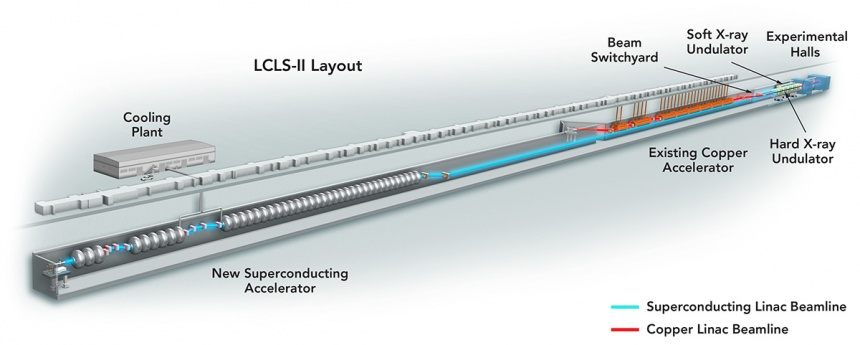
\includegraphics[width=0.99\linewidth]{pic/lcls.jpg}}
		%https://portal.slac.stanford.edu
	\end{minipage}
	\end{figure}
	\raggedright\tiny{\href{http://www.irtnanoelec.fr}{ссылка на рисунок сверху}}\\
	\raggedright\tiny{\href{https://portal.slac.stanford.edu/sites/conf_public/lclsiihe2018/PublishingImages/Forms/AllItems.aspx}{ссылка на рисунок снизу}}
\end{frame}
\fi

\small
\begin{frame}\label{r3}
\frametitle{Карта ускорительных центров}
\begin{figure}[h]
		\center{\includegraphics[width=1.0\linewidth]{pic/map.png}}	
		\raggedright\tiny{Жёлтым цветом обозначены центры синхротронного излучения}
\end{figure}
\end{frame}

\small
\begin{frame}
\frametitle{Сибирский Кольцевой Источник Фотонов}\label{t1}
\begin{figure}[h]
	\center{}
	\begin{minipage}[h]{0.75\linewidth}
		\center{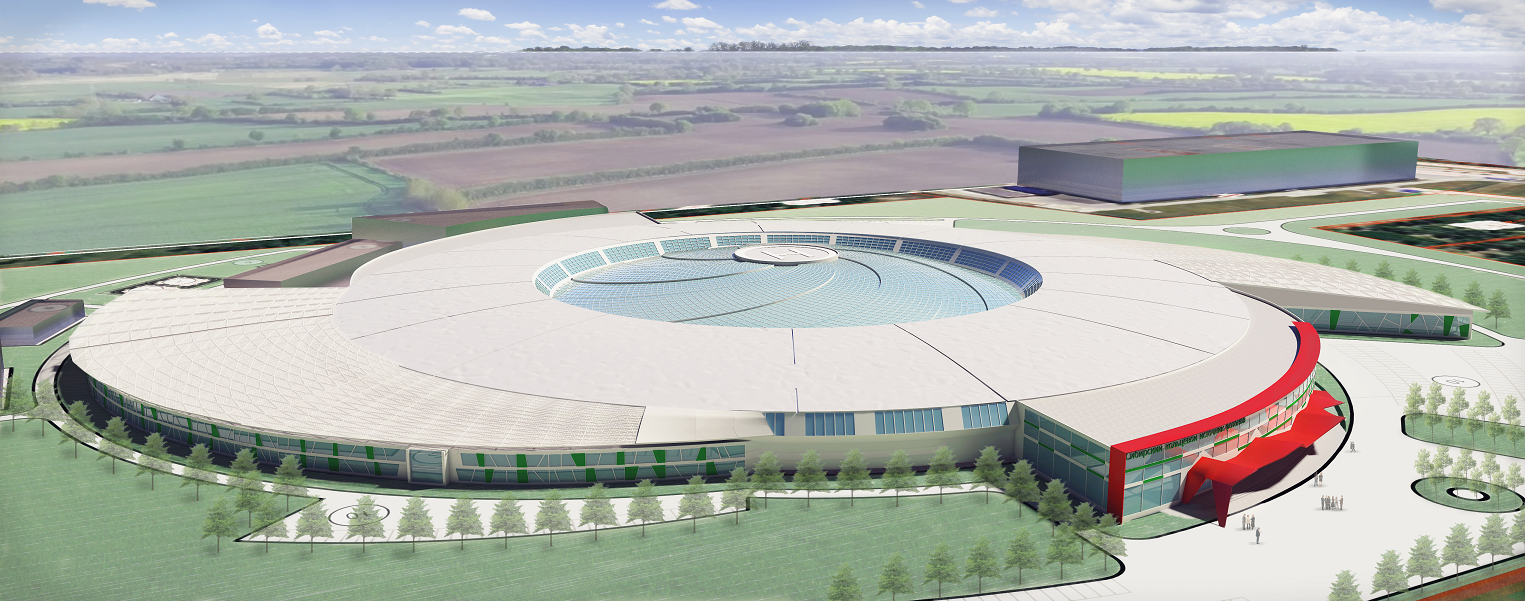
\includegraphics[width=0.99\linewidth]{pic/SKIF_2_2.png}}
		%http://www.irtnanoelec.fr
	\end{minipage}
	
	\hfill
	\center{}
	\begin{minipage}[h]{0.75\linewidth}
		\center{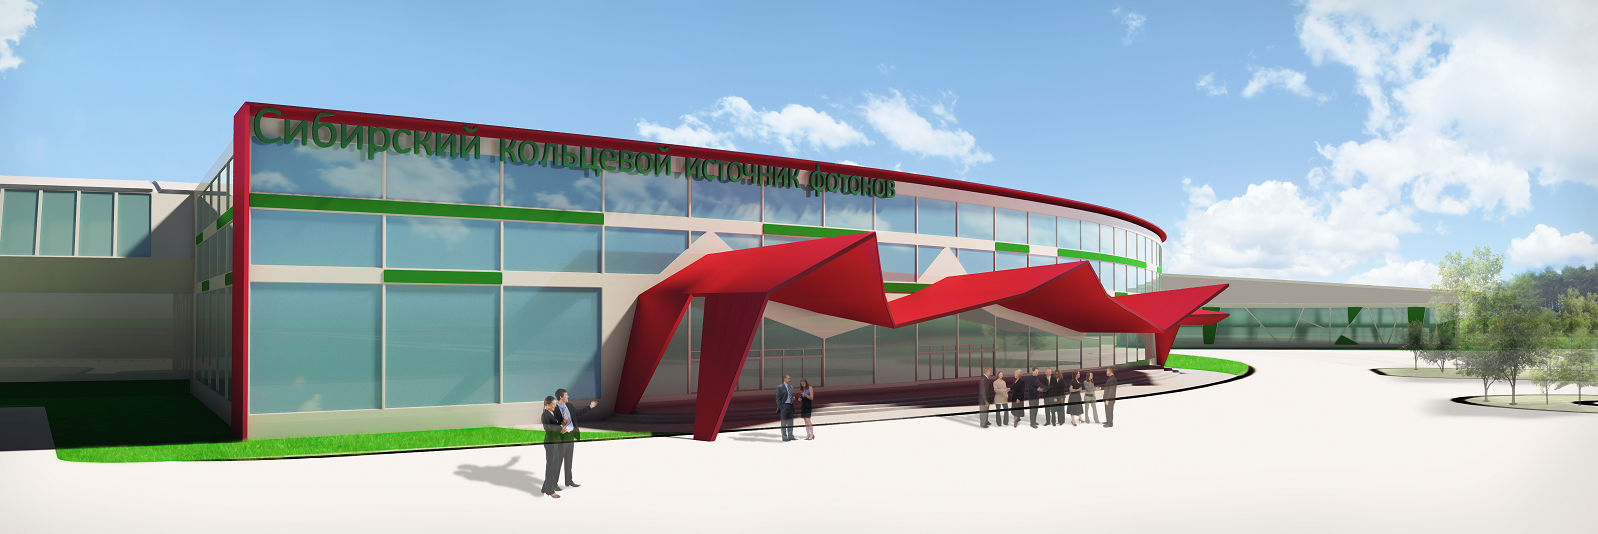
\includegraphics[width=0.99\linewidth]{pic/SKIF_1_2.png}}
		%https://portal.slac.stanford.edu
	\end{minipage}
\end{figure}
\end{frame}

\small
\begin{frame}
\frametitle{Оптическая группа ЦКП <<СКИФ>>}\label{t1}
\begin{figure}[h]
	\center{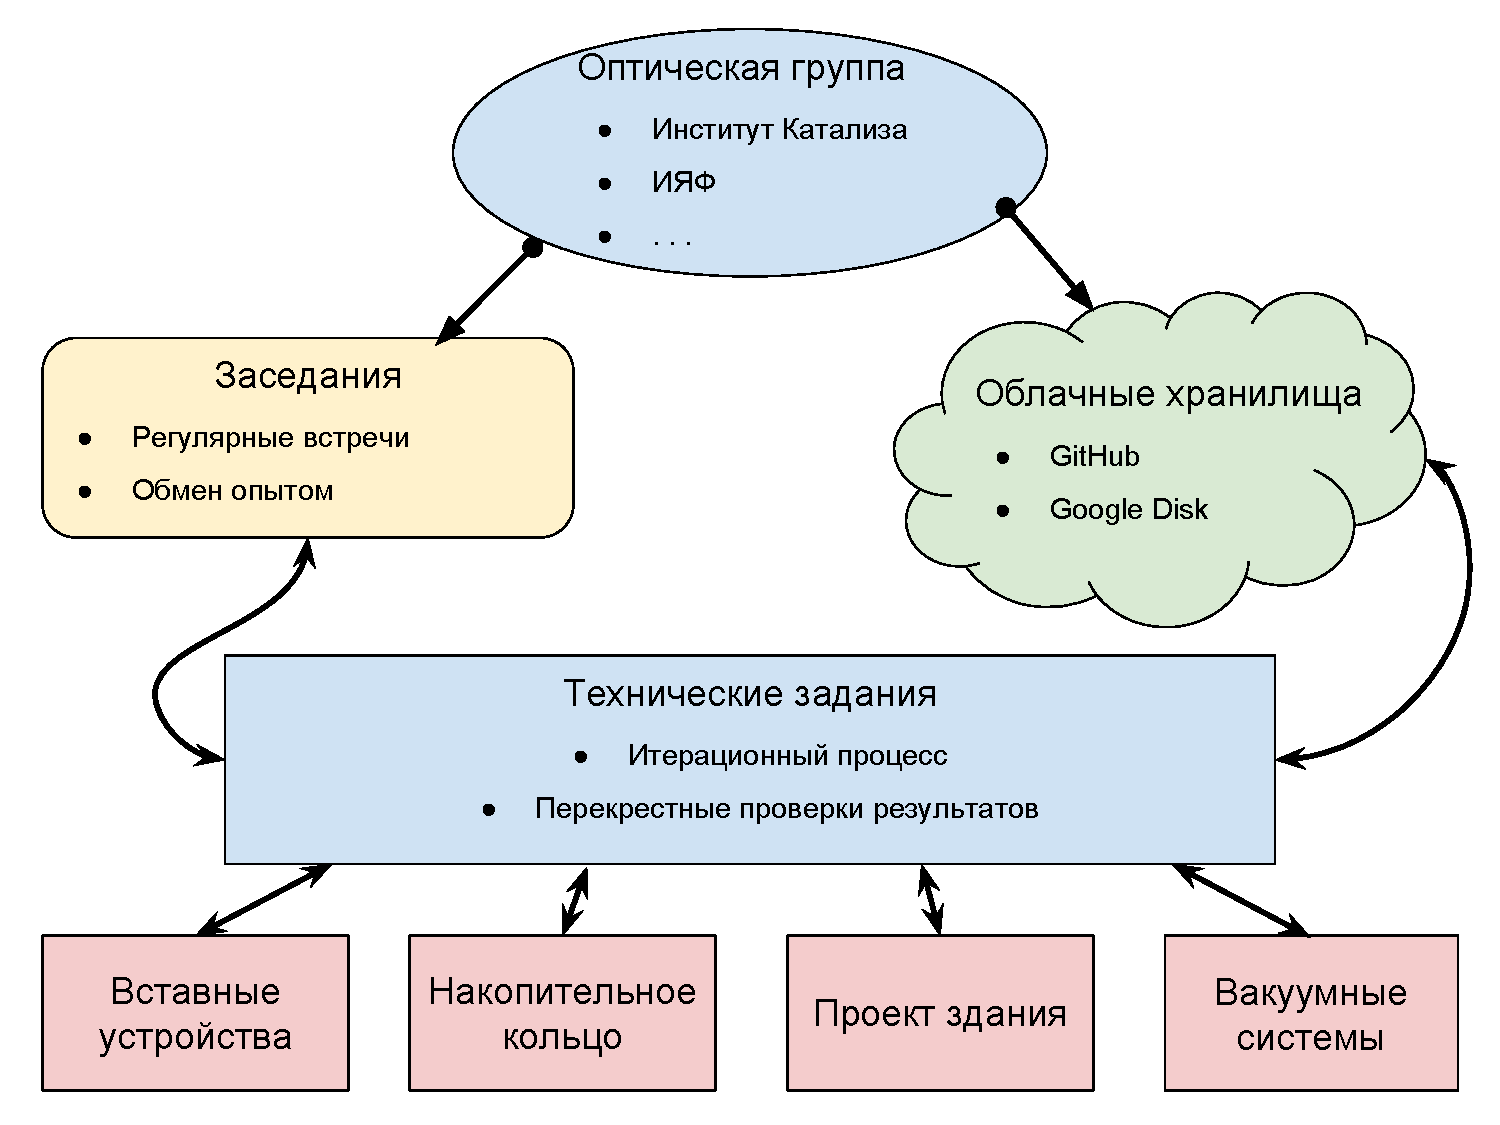
\includegraphics[width=0.8\linewidth]{pic/scheme.pdf}}
\end{figure}
\end{frame}

\small
\begin{frame}
\frametitle{Структура синхротрона}\label{t1}
\vspace{-10pt}
\begin{figure}[h]
	\center{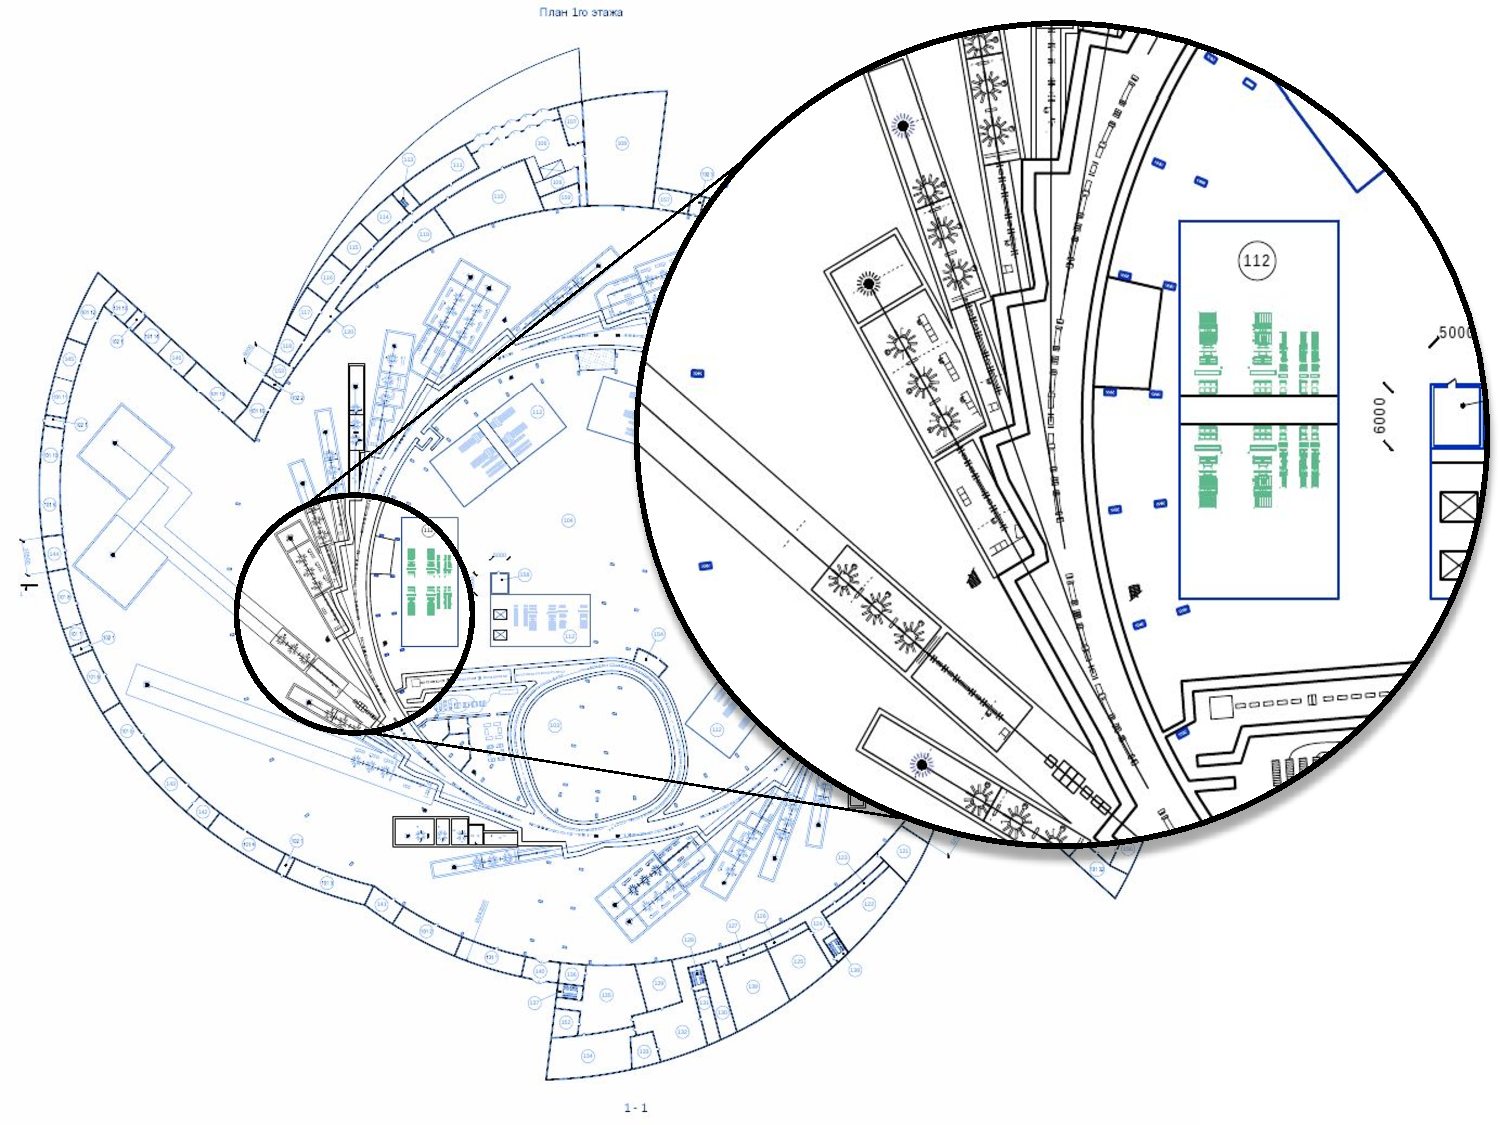
\includegraphics[width=0.95\linewidth]{pic/outline.pdf}}	
\end{figure}
\end{frame}
\iffalse
\vspace{-10pt}
\begin{table}
	\centering
	\begin{tabular}{ccccc}
		\hline
		$\sigma_x, [m]$ 	   & $\sigma_{x'}, [rad]$   & $\sigma_y, [m]$       & $\sigma_{y'}, [rad]$   & $\Delta E / E$      \\ \hline
		$33.0 \times 10^{-6}$  & $2.65 \times 10^{-6}$  &  $8.6 \times 10^{-7}$ & $5.0 \times 10^{-7}$   & $8.6 \times 10^{-4}$ \\ \hline	
	\end{tabular}
\end{table}
\fi

\small
\begin{frame}
\frametitle{SRW. Сред моделирования}\label{t1}
SRW --- Synchrotron Radiation Workshop. Код для моделирования оптических систем.
$\mathnormal{r\omega}$-пространство, ближняя зона.\\
\begin{itemize}
	\item Вставные устройства:\\
\end{itemize}
	\hspace{25pt}$\mathnormal{\vec{\widetilde{E}}_{\bot}(\vec{r}_0, \omega) = 
	\cfrac{i\omega e}{c}\displaystyle\int\limits_{-\infty}^{\infty} dt'\bigg[\cfrac{\vec{\beta} - \vec{n}}{|\vec{r}_0 - \vec{r'}_0(t')|} - \cfrac{ic}{\omega}\cfrac{\vec{n}}{|\vec{r}_0 - \vec{r'}_0(t')|^2}\bigg]\times}$\\
	\hspace{195pt}$\mathnormal{\exp[i\bigg(t' + \cfrac{|\vec{r}_0 - \vec{r'}_0(t')|}{c}\bigg)]}$

\begin{itemize}	
	\item Фурье оптика:\\
	\centering
	\vspace{-10pt}
	$\mathnormal{g_2(x_2, y_2) = \displaystyle\int\limits_{-\infty}^{\infty}\displaystyle\int\limits_{-\infty}^{\infty}
		g_1(\eta, \xi) \ast h(x_2 - \eta, y_2 - \xi)}d\eta d\xi$ \\
	\vspace{-6pt}
	$\Updownarrow$\\
	\vspace{6pt}
	$\mathnormal{G_2(f_x, f_y) = G_1(f_x, f_y)H(f_x, f_y)}$
\end{itemize}
\tiny{\textit{@Oleg Chubar ссылка на \href{https://github.com/ochubar/SRW.git}{GitHub}}}
\end{frame}
%\vec{\widetilde{E}}_{\bot}(\vec{r}_0, \omega) =
%\cfrac{i\omega e}{c}\displaystyle\int\limits_{-\infty}^{\infty} dt'\bigg[\cfrac{\vec{\beta} - \vec{n}}{|\vec{r}_0 - \vec{r'}_0(t')|}-\cfrac{ic}{\omega}\cfrac{\vec{n}}{|\vec{r}_0 - \vec{r'}_0(t')|}\bigg]\\
%\exp[i\bigg(t' + \cfrac{|\vec{r}_0 - \vec{r'}_0(t')|}{c}\bigg)]


\small
\begin{frame}
\frametitle{Ондулятор --- интерференционное устройство}\label{t1}
\begin{figure}[h]
		\center{$\mathnormal{n \lambda_{ph} = s_{ph} - \lambda_u \cos\theta}$}\hspace{10pt}$\longrightarrow$\hspace{10pt}
		{$\mathnormal{\lambda_{ph} = \cfrac{\lambda_{u}}{2n\gamma^2 K}(1 + \cfrac{K^2}{2} + \gamma^2\theta^2)}$}
		\center{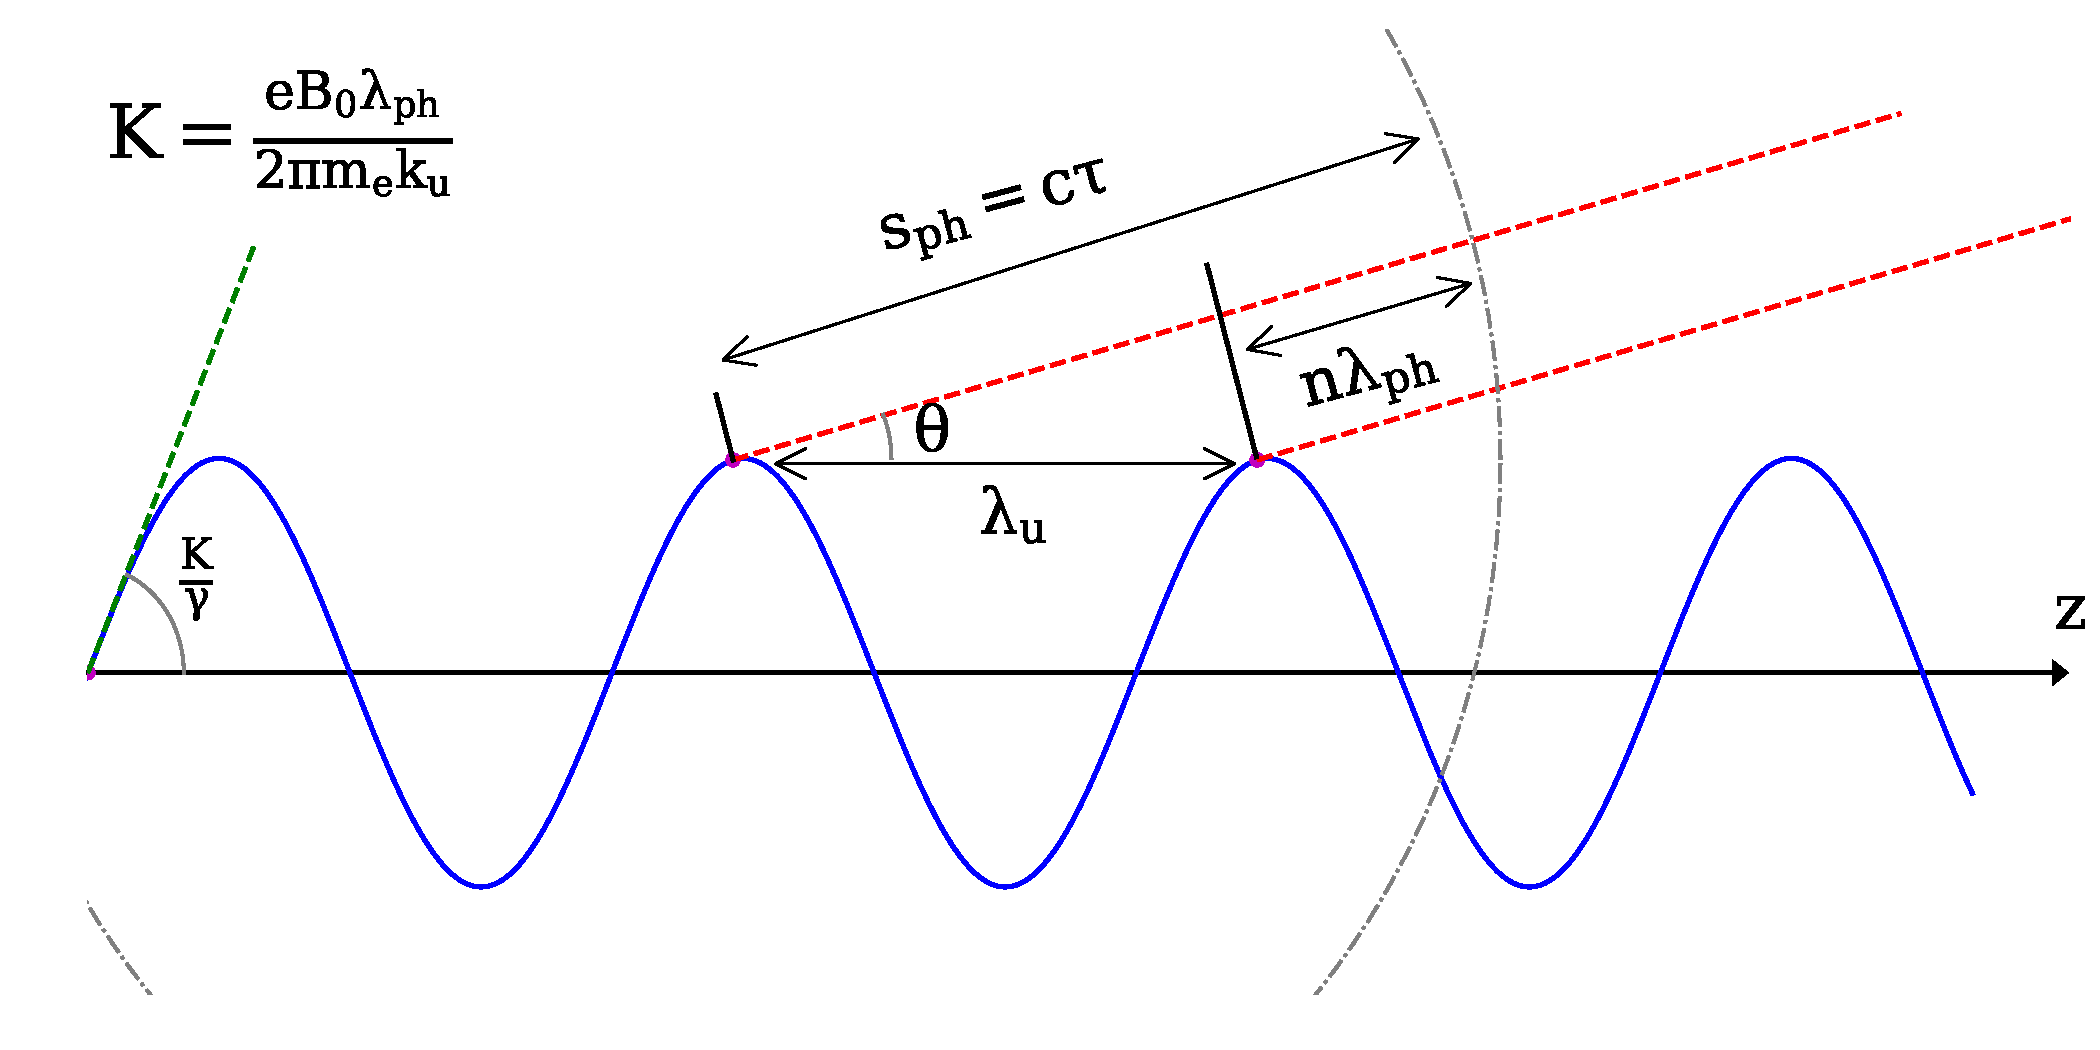
\includegraphics[width=0.99\linewidth]{pic/traj.pdf}}
\end{figure}
\end{frame}

\small
\begin{frame}
\frametitle{Оптическая схема станции 1-1}\label{t1}
\begin{figure}[h]
\end{figure}
\end{frame}

\small
\begin{frame}
\frametitle{Результаты}\label{t1}
\begin{figure}[h]
\end{figure}
\end{frame}

\small
\begin{frame}
\frametitle{Благодарности}\label{t1}
\begin{figure}[h]
\end{figure}
\end{frame}

\begin{frame}
\begin{center}
	\textbf{Благодарю за внимание}
\end{center}
\end{frame}

\small
\begin{frame}
\frametitle{Дополнительные слайды}\label{t1}
\begin{figure}[h]
\end{figure}
\end{frame}

\small
\begin{frame}
\frametitle{Спектр ондулятора}\label{t1}
\begin{figure}[h]
\end{figure}
\end{frame}

\small
\begin{frame}
\frametitle{Угловое распределение}\label{t1}
\begin{figure}[h]
\end{figure}
\end{frame}




\end{document}
